\subsection{Changing the interval helps, but does not repair the rule}
\label{sec:intervalcomparison}
Welch intervals increase fixed-pool coverage at 50 cells by 1.5--5.0
percentage points on the same draws (paired Monte Carlo standard errors
0.23--0.32 points). They also reduce null rejection, but it remains
8.9--30.8\% and every lower confidence endpoint exceeds 5\%.
Detection remains below 80\% even at the upper confidence endpoints.
Wider intervals improve some operating characteristics without satisfying
the joint requirements. This rules out this particular substitution as a
repair at 50 cells; it does not rule out other methods or validate a higher
threshold. Null and alternative evaluation must accompany any proposed repair.

\paragraph{Why detection can fall as cell count rises.}
The apparent detection curve combines effect sensitivity with a changing
false-positive rate. Figure~\ref{fig:precision} reproduces the pooled-draw
trough with greater precision. For KUL3, percentile detection falls from
49.0\% at 50 cells to 44.0\% at 100, then rises to 57.7\% at 800;
null rejection falls from 32.2\% to 20.3\% to 6.5\%. At 50 and 100 cells,
the median sample-based standard error is respectively 0.66 and 0.86 times
the exact pool-conditional standard deviation. The fraction of draws with
that ratio below one half falls from 29.1\% to 7.6\%. These diagnostics
support a loss of spuriously confident rejections as the sampled variance
becomes better represented, before increasing signal-to-noise dominates.
They do not attribute every change to one mechanism. In particular, all-zero
tumour samples occur in only 0.32\% of the 50-cell draws and none at 100:
the trough is not explained by all-zero samples alone.

\begin{figure}[htbp]
\centering
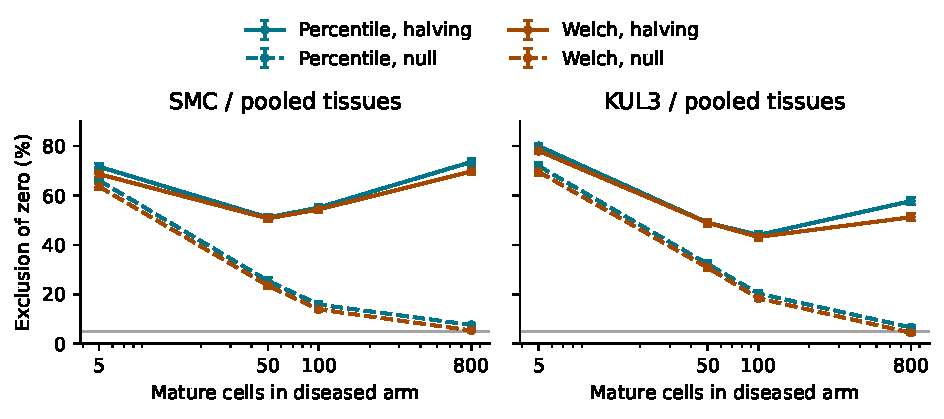
\includegraphics[width=\linewidth]{figures/precision_rejection.pdf}
\caption{Detection must be read alongside null rejection. Pooled-tissue
simulations use 5{,}000 studies per point; bars are 95\% Wilson Monte Carlo
intervals. Solid curves use a halving of expression and dashed curves the
null. The horizontal line marks nominal 5\% rejection. Five-cell intervals
are diagnostic calculations before the reporting gate, which abstains below
20. Both methods use the same samples; their apparent sensitivity at sparse
counts accompanies excessive false positives.}
\label{fig:precision}
\end{figure}

The five-cell diagnostic makes the problem especially clear: pooled
percentile null rejection is 66.1\% in SMC and 71.9\% in KUL3.
Under the halving, 46.2\% and 41.9\% of tumour samples are all zero.
Resampling cannot recover an unobserved positive tail, although the reference
arm still contributes uncertainty. The original reporting gate already
abstains here; the 50-cell failures concern returned answers directly.

\paragraph{Five candidate intervals and a design change, none of which repairs
it.} Substituting the interval is the obvious response, so we tested it rather
than recommending it. On shared draws at 2{,}000 replicates per cell, we
compared the percentile baseline against bootstrap-$t$, BCa, Welch-$t$, a
patient-level cluster bootstrap and a pseudobulk patient-$t$
(Appendix~\ref{app:repair}).

\textbf{Eleven of 144 cells meet the 5\% null target, and all but one are at
800 cells, where the unmodified percentile interval already meets it.} Exactly
one cell has a candidate passing where the baseline fails --- studentised, SMC
reference-only, 100 cells, $5.95\%$ against $6.90\%$ --- a $1.2$ Monte Carlo
standard error gap that reverses at 50 cells. At 50 cells and below all six
fail. Bootstrap-$t$, BCa and Welch-$t$ track the percentile within about
$1.5$ points, because they correct the $z$-versus-$t$ term, which the closed
form values at $0.45$ points.

\textbf{The patient-level candidates never pass anywhere}, and the binding
constraint is the number of clusters the generator supplies rather than the
cells drawn from them: at the committed two-patient holdout --- three
reachable resamples per arm --- the cluster bootstrap abstains on $30$--$47\%$
of draws, and raising the holdout to five patients substitutes uselessness
($0.00\%$ null rejection at $9.15\%$ detection). Balancing the arms rather
than the interval is the one change that helps materially, to
$7.45$--$11.45\%$, and still misses nominal.

\textbf{We therefore prescribe no interval for this design at these
counts}, which is a stronger statement than declining to look.
